\documentclass[a4paper, twocolumn, 10pt]{jarticle}
\usepackage[dvipdfmx]{graphicx}
\usepackage[dvipdfmx]{color}
\usepackage{float}
\usepackage{setspace}
\usepackage[top=20mm,bottom=20mm,left=23mm,right=23mm]{geometry}
\usepackage[hang,small,bf]{caption}
\usepackage{bm}

\usepackage{comment}
%\usepackage[subrefformat=parens]{subcaption}
% \usepackage{jumoline}
\usepackage[hyphens]{url}
\usepackage[dvipdfmx, bookmarkstype=toc, colorlinks=false, pdfborder={0 0 0}, bookmarks=true, bookmarksnumbered=true]{hyperref}
\usepackage{pxjahyper}
\usepackage{here}
\usepackage{otf}

\makeatletter

\def\section{%
	\@startsection{section}{1}{\z@}%
	{.1\Cvs \@plus.1\Cdp \@minus.1\Cdp}%
	{.1\Cvs \@plus.1\Cdp}%
	{\normalfont\normalsize\bfseries}%
}

\def\subsection{%
	\@startsection{subsection}{1}{\z@}%
	{.1\Cvs \@plus.1\Cdp \@minus.1\Cdp}%
	{.1\Cvs \@plus.1\Cdp}%
	{\normalfont\normalsize\bfseries}%
}

\def\@maketitle {
	\begin{center}
		\fontsize{14pt}{0pt}\selectfont
		{\bf \@title}
	\end{center}
	\vspace{1pt}
	\begin{flushleft}
		{指導教員 木村 昌臣}\hfill{片岡 凪}
	\end{flushleft}
	\vspace{10pt}
}

\makeatother

\captionsetup{compatibility=false}
\pagestyle{empty}


\begin{document}

\title{主張と根拠のクラスタを用いた多様な主張を提示するニュース推薦手法の提案}

\maketitle

\thispagestyle{empty}

%%%%%%%%%%%%%%%%%%%%%%%%%%%%%%%%%%%%%%%%%%%
%% Section 研究の背景と目的
%%%%%%%%%%%%%%%%%%%%%%%%%%%%%%%%%%%%%%%%%%%
\section{研究の背景と目的}

ニュース記事となる出来事は,記者によって受け取り方や伝え方が異なる.
RSF(Reporters Sans Frontières)は,政治や文化などの要因によって記者の主張が制限されていることを問題視している\cite{2021_world_press_freedom_index}.
近年のWebニュースには世界中の記者たちの様々な主張が散見されるが,言語の違いによる時間的コストなどから,多くの読者はそれらの主張の一部しか把握できない.

Yangらは,ニュース読者が出来事を正確かつ迅速に把握できるように,
階層的クラスタリングを用いて記事に対するツイートの主張をグループ化する手法を提案した\cite{yang_scalable_2021}.
この研究ではcovid-19の話題に限定した記事について主張をグループ化しているが,この手法をWeb上の無数の話題の記事に適用した場合,無数の話題の主張のグループが生成されることになる.
% 1度のクラスタリングで
% 無数の主張のグループが生成されることになる.
これでは,covid-19のワクチンに対する主張と脳炎のワクチンに対する主張が近くにグループ化されるといった事が起き得るため,同じ出来事の異なる主張の収集に時間を要してしまう.
% 異なる話題の似た主張をグループ化するエラーに繋がりやすいと考えられる.

% 近いグループに正確さ
% カテゴリをcovid-19に限定させたニュースだけでも
% ノイズとなり得る
% Web上には世界の無数の記事には対応できない
% クラスタ数がいうほど減っていない



% より近い出来事を

そこで本研究では,世界のニュース読者の正確かつ迅速な出来事の把握のため,閲覧記事と出来事が類似する世界の記事をグループ化し,同じ出来事のグループから主張が異なる文章を推薦する手法を提案する.図\ref{system_abstract}に提案手法のシステムの概要を示す.
% ここで,「出来事」は記者の解釈に依存しない事象とし,「主張」は記者が伝えるべきだと判断した出来事の解釈とする.

\begin{figure}[H]
	\centering
	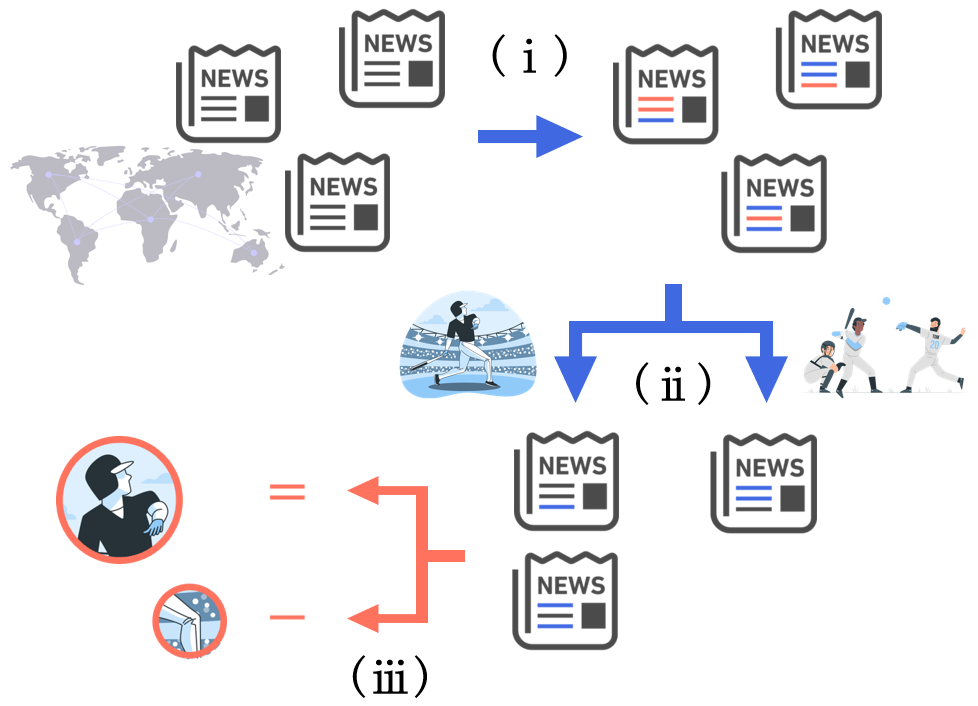
\includegraphics[keepaspectratio, width=60mm]{img/system_abstract.png}
	% 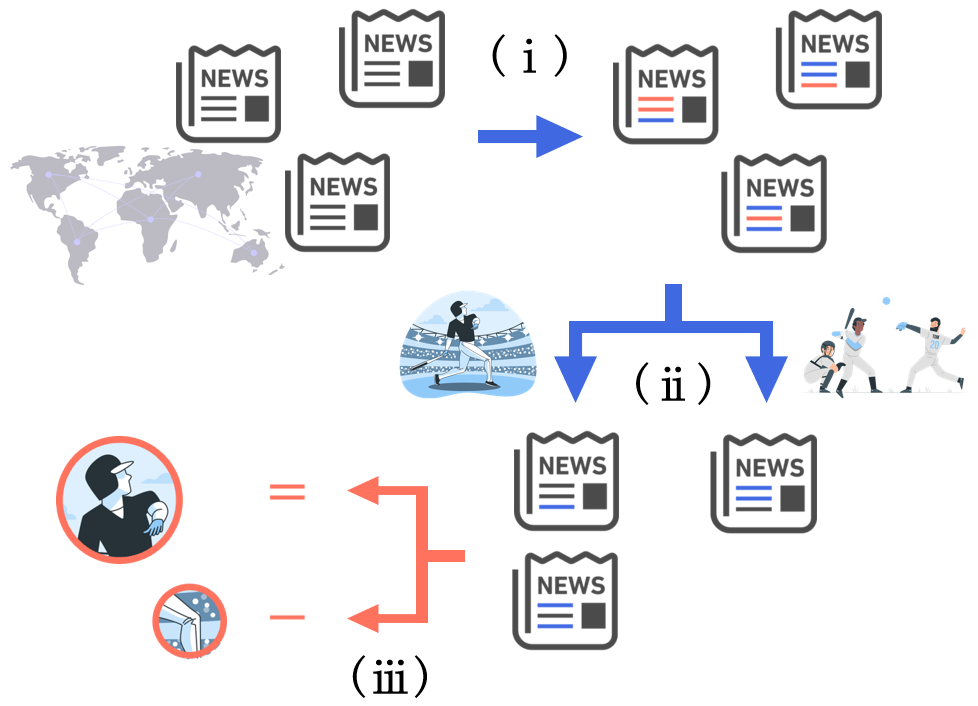
\includegraphics[keepaspectratio, width=60mm]{img/system_abstract.png}
	% 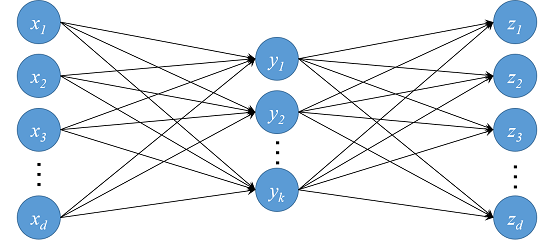
\includegraphics[keepaspectratio, width=60mm]{img/sample.png}
	\caption{
    提案手法のシステムの概要
    \\$\rm(\hspace{.18em}i\hspace{.18em})$
    記事の文章を出来事の文と主張の文に分類
    \\$\rm(\hspace{.08em}ii\hspace{.08em})$
    出来事の文章の類似度で記事をクラスタリング
    \\$\rm(i\hspace{-.08em}i\hspace{-.08em}i)$
    主張の文の類似度で主張の文をクラスタリング
  }
	\label{system_abstract}
\end{figure}


%%%%%%%%%%%%%%%%%%%%%%%%%%%%%%%%%%%%%%%%%%%
%% Section 関連研究
%%%%%%%%%%%%%%%%%%%%%%%%%%%%%%%%%%%%%%%%%%%
% \section{関連研究}
% 意味や話題が類似する文章の推薦手法として,LDA(Latent Dirichlet Allocation)~\cite{tian_labeled_2018}やSentence-BERT~\cite{reimers_sentence-bert_2019}が提案されている.
% LDAは記事に関連の深い単語群とそれぞれの単語の関連度を出力するが,単語群同士の関係性が得られないという点で,出来事の類似度が高い記事は得にくいと考えられる.
% 一方,Sentence-BERTは単語同士の関係性を加味した文意の数値ベクトルを出力するため,より高い出来事の類似度が得られると考えられる.
% しかし,記事の全文をSentence-BERTに入力した場合,出来事の類似度の算出に主張を述べる文も考慮することになり,より近い出来事に関する主張の違いを推薦できない.

% \begin{comment}
% SCDV, オントロジー, Transformer
% 潜在的意味,同義語
% トピック同士の関係が考慮されない
% 多言語に対応していない
% 主張に着目した研究は少ない
% 事象と主張が混在
% \end{comment}

% \begin{table}[h]
%   \caption{キャプション}
%   \label{table_a}
%   \centering
%   \begin{tabular}{lcr}
%     \hline
%     手法   & 正解率[\%]  &  計算時間[ms]  \\
%     \hline \hline
%     手法A  & 92.3  & 512 \\
%     手法B  & 87.4  & 32  \\
%     \hline
%   \end{tabular}
% \end{table}

%%%%%%%%%%%%%%%%%%%%%%%%%%%%%%%%%%%%%%%%%%%
%% Section 提案手法
%%%%%%%%%%%%%%%%%%%%%%%%%%%%%%%%%%%%%%%%%%%

\section{提案手法}

% \subsection{データセットの選定と前処理}
\subsection{RoBERTaによる出来事の文と主張の文の分類}

まず,英文以外の記事をDeepL APIで英訳して用いる.
% このとき
% また,記事の出来事をより類似させるため,同じ出稿日の記事を扱う.
% の各文章が,出来事と主張のどちらを述べているかを分類する.
本研究では,記事の文章が出来事を述べる文と主張を述べる文に二分できると仮定する.
そして,出来事の文のみ,主張の文のみで2回に分けてクラスタリングすることで,より近い出来事に関する異なる主張の文の推薦を目指す.

出来事と主張の文の分類には,Transformerを応用した分類器を用いる.Transformerは入力文から翻訳後の文を予測するような機械学習モデルであるが,Dense層を加えたモデルのエンコード部分を用いることで分類タスクに応用できる.
% 入力部分にDense層を付加
本研究では,入力文を数値ベクトルに変換するために,多くのニュース記事を事前学習したRoBERTaを用いる.
また,分類器の学習には,英文をEvidenceを述べるかClaimを述べるかでラベル付けしたIBMのDebater Datasetsを用いる~\cite{debater_datasets}.

% この分類は,記事で二重引用符が用いられる際に様々な人物・組織が主張を述べている傾向があることに基づく.
% ここで,世界の記事でこの分類を行うために,Transformerを用いた分類モデルを作成し,仮定した分類基準を教師ラベルとして英語の記事で学習する.
% Transformerの単語埋め込みには,多くのニュース記事を事前学習したRoBERTaを用いる.
% また,多言語の引用符に相当する文構造を学習するため,二重引用符を除去した英語の記事を入力する.
% その後,世界の記事を英語に機械翻訳し,学習したモデルで各文章が主張を述べる文章か否かを分類する.

次に,出来事の文をSentence-BERTを用いて数値ベクトルに変換し,それらのコサイン類似度を基に記事のクラスタリングを行う.
% このとき,出来事の意味が階層構造を持つと仮定し,Ward法で階層的クラスタリングを行う.
最後に,閲覧記事が属するクラスタの主張の文を抽出し,
% 同様にSentence-BERT,コサイン類似度,ward法を用いて文章の
クラスタリングを行う.


% 最後に,得たそれぞれのクラスタ内の記事に対し,主張を述べる文章の意味を基に,再びTransformerで記事のクラスタリングを行う.
% Transformerの単語埋め込みには,クラスタリングに特化したSentence-BERTを用いる.
% 以上の操作を記事を閲覧した際に実行することにより,閲覧した記事と出来事が類似し,主張が異なる世界の文章を得ることができる.

% 主張の細かい違いに

% (追加候補)
% Transformerの埋め込みの種類\\
% Transformerの詳しいクラスタリング手法(Sentence-BERT)\\
% SCDV(文章分散表現)\\
% オントロジー\\
% 単語埋め込みはRoBERTa

% 世界のニュース記事
% 代弁
% 同じトピック,異なる

% 全貌がわからない 偏見

% を主張とし,
% 事象と主張を分け
% この順に分割

%%%%%%%%%%%%%%%%%%%%%%%%%%%%%%%%%%%%%%%%%%%
%% Section 研究状況
%%%%%%%%%%%%%%%%%%%%%%%%%%%%%%%%%%%%%%%%%%%
\section{研究状況}

分類精度の確認のため,前述の操作で出来事の文と主張の文の分類を行った.
ただし,分類する日本の記事にはJapanese FakeNews Dataset中の偽物でないWikinewsを利用した~\cite{japanese_fakenews_dataset}.
% 簡単のために出稿日は統一していない.
学習で正解率が約0.993となったモデルで分類を行ったところ,表\ref{classify_result}の結果が得られた.


\begin{table}[h]
  \caption{Evidenceの文 ($E$) とClaimの文 ($C$) の分類結果}
  \label{classify_result}
  \centering
  \begin{tabular}{cp{6cm}}
    \hline
    分類 & \multicolumn{1}{c}{翻訳前の入力文(一部抜粋)}  \\
    \hline \hline
%     E  & また毎日新聞によると,脇谷は「4試合で10分くらいしか試合に出ていない \\
    $E$  & 決勝のヒットを打った23日の試合も1球だけで終わった \\
    $C$  & 日本シリーズ進出を決めてうれしい \\
%     $C_3$  & 日本一になりたい」と喜びと抱負を述べた \\
%     $E_4$ & 一方,敗れた中日・落合博満監督は「今年1年は思いがけない風が吹きっぱなしだった\\
%     $C_5$  & 負けたけども伸びしろはある \\
%     C  & 来年は逆転する可能性がある」と話している \\
    \hline
  \end{tabular}
\end{table}

% また毎日新聞によると,脇谷は「4試合で10分くらいしか試合に出ていない
% 決勝のヒットを打った23日の試合も1球だけで終わったまた毎日新聞によると,脇谷は「4試合で10分くらいしか試合に出ていない 
% 日本シリーズ進出を決めてうれしい
% 日本一になりたい」と喜びと抱負を述べた
% 一方,敗れた中日・落合博満監督は「今年1年は思いがけない風が吹きっぱなしだった
% 負けたけども伸びしろはある
% 来年は逆転する可能性がある」と話している

% evidence:   According to the Mainichi Shimbun, Wakitani also said, "I've only played about 10 minutes in four games
% evidence:   Even the game on the 23rd, in which I got the final hit, ended with just one pitch
% claim   :   I'm happy to have made it to the Japan Series
% claim   :   I want to be the best in Japan," he said, expressing his joy and aspirations
% evidence:   On the other hand, Hiromichi Ochiai, manager of the defeated Chunichi team, said, "This year has been full of unexpected winds
% claim   :   We lost, but we have room to grow
% claim   :   There is a possibility that we can turn things around next year

% \begin{figure}[h]
%   \centering
%   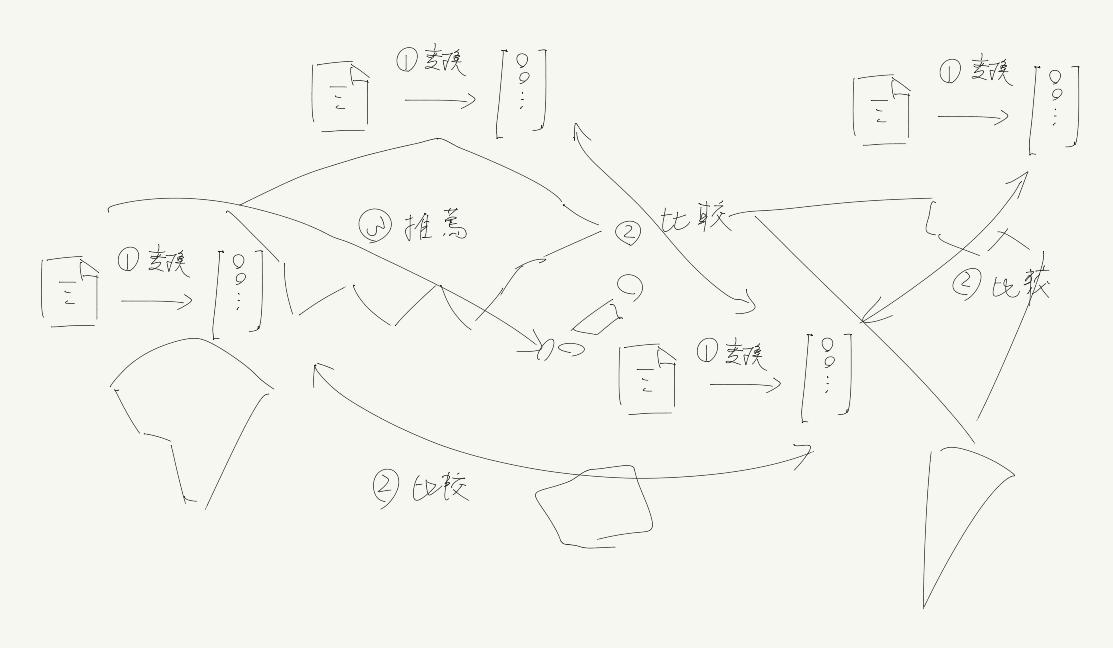
\includegraphics[keepaspectratio, width=70mm]{img/abstract_v01.PNG}
%   \caption{仮図(分類結果の図にする予定)}
%   \label{fig_01}
% \end{figure}

文$E$は,記者の解釈に依存しない,誰が観測しても不変な出来事を表している.
また,文$C
% , C_3, C_5
$は,出来事に対する主張を表している.
一方で
% 文$E_4$は
,
% 1年間の出来事に対する監督の解釈を記者が取り上げたものであり,出来事を表しているとは捉えにくい.
% 分類エラーの要因としては,
% 文中に出来事を表す「敗れた」という言葉が含まれることや,「風が吹く」という出来事を表す言葉で主張を述べるような例外が存在することが挙げられる.
文中に出来事を表す「敗れた」や「風が吹く」という言葉が含まれることより,出来事を誤分類したケースも見られた.

%%%%%%%%%%%%%%%%%%%%%%%%%%%%%%%%%%%%%%%%%%%
%% Section 今後の予定
%%%%%%%%%%%%%%%%%%%%%%%%%%%%%%%%%%%%%%%%%%%
\section{今後の予定}

今後は,1文中の出来事と主張の要素を比率で考えるなどして,推薦精度を高めるように研究を進める予定である.

% 現在,主張を述べる文章を二重引用符を含む文章と仮定しているが,指示語や否定語の係り受けや引用符内の単語数によってはこの仮定は不適切である可能性がある.
% また,引用符の外の文章も主張を述べる文章である可能性があり,推薦の精度のために精査が必要である.
% 加えて,Transformerに代わるクラスタリング手法として,文意をベクトルで表現するLCDA(Sparse Composite Document Vectors)の利用も検討している.
% LCDAもまた主張の類似度を測るための手法ではないため,Trandsformerとのクラスタリングの精度の比較が必要である.

% を用いた → で

% (事象と主張以外の集合が存在する可能性)
\begin{comment}
LCDAの組み込み
LCDAとの比較
””の種類
””以外の主張
翻訳の代わりに再現性のある多言語トピック分析rectr
Transformerのpredictが遅かった(並列処理したら速い?)
\end{comment}

\cite{blei_latent_nodate}

\bibliographystyle{junsrt}
{\footnotesize \bibliography{ref.bib}}

\end{document}
